% !TeX root = RJwrapper.tex

\title{\pkg{ordinalClust}: An R Package to Analyze Ordinal Data}
\author{by Margot Selosse, Julien Jacques and Christophe Biernacki}

\maketitle

\abstract{
Ordinal data are used in many domains, especially when measurements are collected from people through observations, tests, or questionnaires. \CRANpkg{ordinalClust} is an innovative R package dedicated to ordinal data that provides tools for modeling, clustering, co-clustering and classifying such data. Ordinal data are modeled using the BOS distribution, which is a model with two meaningful parameters referred to as "position" and "precision". The former indicates the mode of the distribution and the latter describes how scattered the data are around the mode: the user is able to easily interpret the distribution of their data when given these two parameters. The package is based on the co-clustering framework (when rows and columns are simultaneously clustered). The co-clustering approach uses the Latent Block Model (LBM) and the SEM-Gibbs algorithm for parameter inference. On the other hand, the clustering and the classification methods follow on from simplified versions of the SEM-Gibbs algorithm. 
%Indeed, the clustering can be seen as a simpler co-clustering whose column-clusters do not have to be found. In the same way, classification can be seen as a simpler co-clustering whose row-clusters do not have to be found on the training set. 
For the classification process, two approaches are proposed. In the first one, the BOS parameters are estimated from the training dataset in the conventional way. In the second approach, parsimony is introduced by estimating the parameters and column-clusters from the training dataset. We empirically show that this approach can yield better results. For the clustering and co-clustering processes, the ICL-BIC criterion is used for model selection purposes. 
An overview of these methods is given, and the way to use them with the \pkg{ordinalClust} package is described using real datasets. 
The latest stable package version is available on the Comprehensive R Archive Network (CRAN).
}

\section{Introduction}
Ordinal data is a specific kind of categorical data occurring when the levels are ordered \citep{Agresti12}. Some common contexts for the collection of ordinal data include satisfaction surveys, aptitude and personality tests and psychological questionnaires. In the present work, an ordinal variable is represented by $x$ and it is considered to have $m$ levels that are written $\left(1,...,m\right)$.

Thus far, ordinal data have received more attention from a supervised point of view. For example: a marketing firm investigating which factors influence the size of a soda (small, medium, large or extra large) that people order at a fast-food chain. These factors may include which type of sandwich is ordered (burger or chicken), whether or not fries are also ordered, and the consumer's age. In this case, an observation consists in factors of different types and the variable to predict is an ordinal variable. Several software can analyze ordinal data in a regression framework. The cumulative link model (CLM) assumes that:

\begin{center}
$\mbox{logit}\left(p\left(x\leq \mu\right)\right)=\log\frac{p\left(x\leq \mu\right)}{1-p\left(x\leq \mu\right)} = \beta_{0}\left(\mu\right) + \boldsymbol{\beta}^t\boldsymbol{t}$,
\end{center}

\noindent where $x$ is the ordinal variable, $\mu$ is one of its levels, $\boldsymbol{t}$ are the covariates, and $\beta_0 \left(1\right) \leq \beta_0 \left(2\right) \leq \ldots \leq \beta_0 \left(m\right)$ . In the absence of covariates, it is equivalent to a multinomial model. 
CLMs are a powerful model class for ordinal data since observations are handled as categorical, their ordered nature is exploited and the regression framework enables interpretable analyses. In R, several packages implement this kind of models. The package \CRANpkg{MASS} \citep{venables2002} implements the CLM with standard link functions, while \CRANpkg{VGAM} \citep{Yee2010}, \CRANpkg{rms} \citep{harrell2018}, \CRANpkg{brms} \citep{burkner17} and \CRANpkg{ordinal} \citep{Christensen15} bring additional functions and features. Other contributions implement algorithms for ordinal data classification. For instance, the \CRANpkg{ordinalForest} package \citep{Hornung19,Hornung19b} uses ordinal forests and \CRANpkg{monmlp} \citep{cannon17} uses neural networks, both to predict ordinal response variables. Finally, the \CRANpkg{ocapis} package \citep{Gomez2019} implements several methods (such as CMLs, Support Machine, Weighted k-Nearest-Neighbor) to classify and preprocess ordinal data.

However, the focus of these techniques differs from ours in two ways. Firstly, they work in a supervised framework (classification). Secondly, they work with datasets for which the variables to predict are ordinal responses: the other variables are of various types. Our goal is to provide a tool for unsupervised and supervised tasks, and for datasets comprised only of ordinal variables only (in the classification context, the response is categorical). From an unsupervised point a view, the Latent Gold Software \cite{Vermunt06} is -- to our knowledge -- the only software that uses the CMLs to cluster the data. Nevertheless, the implementation of this method is known to be computationally expensive. In addition, it is not provided through a user-friendly R package.  

Other contributions have defined clustering algorithms with ordinal variables. In \cite{McParland2013}, the authors propose a model-based technique by considering the probability distribution of ordinal data as a discretization of an underlying continuous variable. This approach is implemented in the \CRANpkg{clustMD} package \citep{mcparland17}, which is generally more for heterogeneous data. In \cite{Ranalli16}, the categorical variables are seen as a discretization of an underlying finite mixture of Gaussians.  
In other works, the authors use the multinomial distribution to model the data. For instance in the case of \cite{Giordan11}, the multinomial distribution and a cluster tree are used, whereas \cite{jollois09} apply a constrained multinomial distribution. However, these contributions do not provide a way to co-cluster and classify ordinal data. Furthermore, they are not always available as an R package (except in the case of \cite{McParland2013}). More recently, \cite{Corneli20} proposed a method to co-cluster ordinal data modeled via latent Gaussian random variables. Their package \CRANpkg{ordinalLBM} \citep{Corneli2020b} is available on CRAN.

Finally, the CUB (Combination of a discrete Uniform and a shifted Binomial random variable) model \citep{Piccolo2003} is widely used to analyze ordinal datasets. For instance, \cite{corduas2008} proposes a clustering algorithm based on a mixture of CUB models. In the CUB model, an answer is interpreted as the result of a cognitive process where the decision is intrinsically continuous but is expressed on a discrete scale of $m$ levels. This approach interprets the choice of the respondent as a weighted combination of  two components. The first component reflects a personal feeling and is expressed by a shifted binomial random variable. The second component reflects an intrinsic uncertainty and is expressed by a uniform random variable. Many extensions for the CUB model have been defined and the \CRANpkg{CUB} package \citep{Simone18} implements the associated statistical methods.
%The aim of the package \pkg{ordinalClust} is to provide a model-based set of functions to perform clustering, co-clustering and classification on ordinal datasets. 

More recently, \citet{biernacki16} proposed the so-called Binary Ordinal Search model, referred to as the "BOS" model. It is a probability distribution specific to ordinal data that is parameterized with meaningful parameters $(\mu,\pi)$, linked to a position and precision role, respectively. This work also describes how the BOS distribution can be used to perform clustering on multivariate ordinal data. \citet{jacques17} then employed this distribution coupled to the Latent Block Model \citep{Govaert2003} in order to carry out a co-clustering on ordinal data. The co-clustering task consists of simultaneously clustering the rows and the columns of the data matrix. It is a useful way of clustering the data while introducing parsimony, and providing more interpretable partitions. The authors in \cite{jacques17} showed that their algorithm can easily deal with missing values. However, this model could not take ordinal data with different numbers of levels into account. \citet{Selosse18} used an extension of the Latent Block Model to overcome this issue. These works have proved their proficiency and also provide efficient techniques to perform clustering and co-clustering of ordinal data. The purpose of the \pkg{ordinalClust} package is to offer a complete tool for analyzing ordinal data by implementing these methods. Furthermore, it presents a novel approach for classifying ordinal datasets with categorical responses. The present document gives an overview of the underlying methods and illustrates usage of \pkg{ordinalClust} through concrete examples. The paper is organized as follows. In the section~"\nameref{sec:stat-methods}", the notation and models are described. The section~"\nameref{sec:appli}" presents the functions of \pkg{ordinalClust} and details a use case for psychological survey datasets. The section~"\nameref{sec:conclusion}" discusses the limits of \pkg{ordinalClust} and future work for the package.


\section{Statistical methods}
\label{sec:stat-methods}
\subsection{Data Notation}
A dataset of ordinal data will be written as $\boldsymbol{x}=\left(x_{ij}\right)_{i,j}$, with $1 \leq i \leq N$ and $1 \leq j \leq J$, $N$ and $J$ denoting the number of individuals and the number of variables, respectively. Furthermore, a dataset can contain missing data. While dealing with this aspect, the dataset will be expressed by $\boldsymbol{x} =\left(\boldsymbol{\check{x}},\boldsymbol{\hat{x}}\right)$, with $\boldsymbol{\check{x}}$ being the observed data and $\boldsymbol{\hat{x}}$ being the missing data. Consequently an element of $\boldsymbol{x}$ will be annotated as follows:
$
\check{x}_{ij}\text{, whether }{x}_{ij}\text{ is observed, }\hat{x}_{ij}\text{ otherwise}
$. 


\subsection{The BOS model}
\label{sec:BOS}
The BOS model \citep{biernacki16} is a probability distribution for ordinal data parameterized by a position parameter $\mu \in \{1,...,m\}$ and a precision parameter $\pi \;\in\; [0,1]$. It was built on the assumption that an ordinal variable is the result of a stochastic binary search algorithm within the ordered table $\left(1,...,m\right)$. This distribution rises from a uniform distribution when $\pi=0$ to a more peaked distribution around the mode $\mu$ when $\pi$ grows, and reaches a Dirac distribution at the mode $\mu$ when $\pi=1$. Figure~\ref{fig:bos} illustrates the shape of the BOS distribution with different values of $\mu$ and $\pi$. In \citet{biernacki16} it is shown that the BOS distribution is a polynomial function of $\pi$ with degree $m-1$ whose coefficients depend on the position parameter $\mu$. For a univariate ordinal variable, the path in a stochastic binary search can be seen as a latent variable. Therefore, an efficient way to perform the maximum likelihood estimation is through the EM algorithm \citep{Dempster77}.

\begin{figure}[ht!]
\centering
  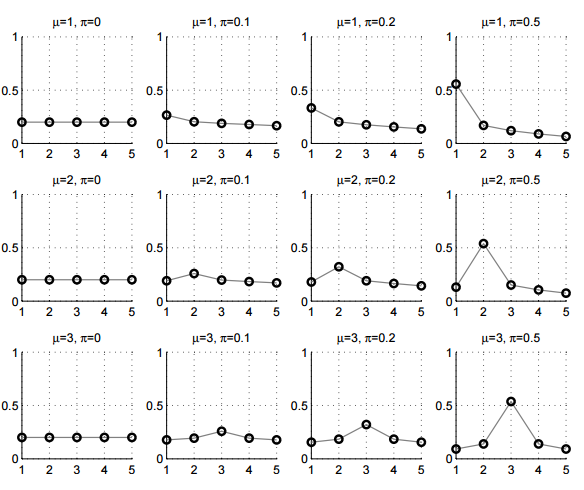
\includegraphics[width = .7\textwidth]{images/BOS.PNG}
    \caption{BOS distribution $p\left(x;\mu,\pi\right)$: shapes for $m\;=\;5$ and for different values of $\mu$ and $\pi$.}
    \label{fig:bos}
\end{figure}

\subsection{The co-clustering model}
\label{sec:coclust}

\paragraph{Notation}
With this being in a co-clustering context, it is assumed that there are $G$ row-clusters and $H$ column-clusters inherent to the $\boldsymbol{x}$ matrix. It is therefore useful to introduce $g$ (or $h$) which represents the $g^{th}$ (or $h^{th}$) row-cluster (or column-cluster), with $1 \leq g \leq G$ (or $1 \leq h \leq H$). In addition, the sums and the products related to rows, columns, row-clusters and column-clusters will be subscripted using the letters $i$, $j$, $g$ and $h$ respectively.  Therefore, the sums and products will be written as $\underset{i}{\sum}$, $\underset{j}{\sum}$, $\underset{g}{\sum}$ and $\underset{h}{\sum}$, and $\underset{i}{\prod}$, $\underset{j}{\prod}$, $\underset{g}{\prod}$ and $\underset{h}{\prod}$.

\paragraph{Latent Block Model}
Let us consider the data matrix $\boldsymbol{x} = \left(x_{ij}\right)_{i,j}$. It is assumed that there are $G$ row-clusters and $H$ column-clusters that correspond to a partition $\boldsymbol{v}=\left(v_{ig}\right)_{i,g}$ and a partition $\boldsymbol{w}=\left(w_{jh}\right)_{j,h}$ respectively, with $1\leq g \leq G$ and $1\leq h \leq H$. We have noted that $v_{ig}=1$ if $i$ belongs to cluster $g$, whereas $v_{ig}=0$  otherwise, and $w_{jh}=1$ when $j$ belongs to cluster $h$, but $w_{jh}=0$ otherwise. Each element $x_{ij}$ is considered to be generated under a parameterized probability density function $p\left(x_{ij};\alpha_{gh}\right)$. Here, $g$ denotes the cluster of row $i$, and $h$ denotes the cluster of column $j$, while $\alpha_{gh}$ represents the parameters of a probability density function of block $\left(g,h\right)$, a block being the crossing of both a row-cluster and a column-cluster. Figure~\ref{fig:ex-coclustering} is an example of co-clustering performed on an ordinal data matrix.

\begin{figure}[ht!]
\centering
  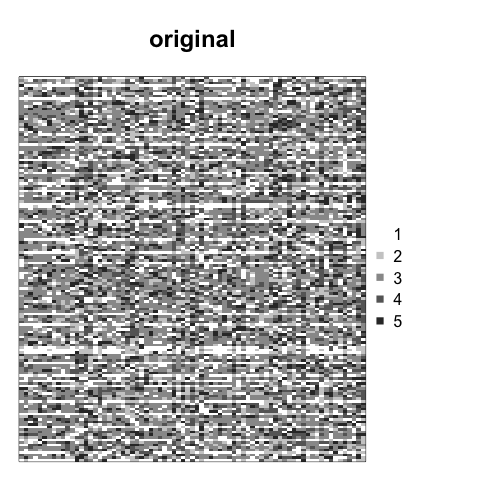
\includegraphics[width = .48\textwidth]{images/ex-original.png}
  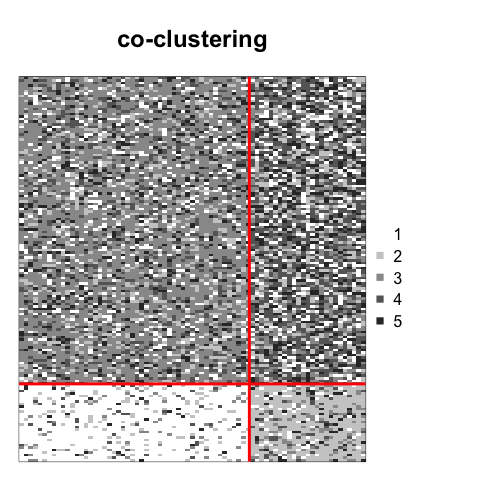
\includegraphics[width = .48\textwidth]{images/ex-coclust.png}
    \caption{Left: original dataset made of ordinal data with $m=5$. Right: a co-clustering is performed with $G=H=2$, the rows and columns are sorted by row-clusters and column clusters, which emphasizes a structure in the dataset.}
    \label{fig:ex-coclustering}
\end{figure}

The univariate random variables $x_{ij}$ are assumed to be conditionally independent given the row and column partitions $\boldsymbol{v}$ and $\boldsymbol{w}$. Therefore, the conditional probability density function of $\boldsymbol{x}$ given $\boldsymbol{v}$ and $\boldsymbol{w}$ can be written as:
\begin{center}
$
  p\left(\boldsymbol{x}|\boldsymbol{v},\boldsymbol{w};\boldsymbol{\alpha}\right) \;=\;
    \underset{i,j,g,h}{\prod}p\left(x_{ij};\alpha_{gh}\right)^{v_{ig}w_{jh}}
$,
\end{center}
where $\boldsymbol{\alpha}=\left(\alpha_{gh}\right)_{g,h}$ is the distribution's parameters of block $\left(g,h\right)$.
Any univariate distribution can be used with respect to the kind of data (e.g: Gaussian, Bernoulli, Poisson...). In the \pkg{ordinalClust} package, the BOS distribution is employed, thus $\alpha_{gh} = \left(\mu_{gh}, \pi_{gh}\right)$. For convenience, the label of row $i$ is also denoted by $\boldsymbol{v}_{i}=\left(v_{i1},...,v_{iG}\right) \in \{0,1\}^{G}$. Similarly, the label of column $j$ is denoted by $\boldsymbol{w}_{j}=\left(w_{j1},...,w_{iH}\right) \in \{0,1\}^{H}$. These latent variables $\boldsymbol{v}$ and $\boldsymbol{w}$ are assumed to be independent so $p\left(\boldsymbol{v},\boldsymbol{w};\boldsymbol{\gamma},\boldsymbol{\rho}\right) \;=\; p\left(\boldsymbol{v};\boldsymbol{\gamma}\right)p\left(\boldsymbol{w};\boldsymbol{\rho}\right)$ with: 
  \begin{center}
  $
    p\left(\boldsymbol{v};\boldsymbol{\gamma}\right)  \;=\;  
    \underset{i,g}{\prod}\gamma_{g}^{v_{ig}} \; \text{ and } \;
    p\left(\boldsymbol{w};\boldsymbol{\rho}\right)  \;=\; 
    \underset{j,h}{\prod}\rho_{h}^{w_{jh}}
  $,
  \end{center}
\noindent with the knowledge that $\gamma_g = p\left(v_{ig}=1\right)$ with ${g \in \{1,...,G\}}$ and  $\rho_h = p\left(w_{jh}=1\right)$ with $h \in \{1,...,H\}$. This implies that, for all $i$, the distribution of $\boldsymbol{v}_i$ is the multinomial distribution $\mathcal{M} \left(\gamma_1,...,\gamma_G\right)$ and does not depend on $i$. In a similar way, for all $j$, the distribution of $\boldsymbol{w}_j$ is the multinomial distribution $\mathcal{M} \left(\rho_1,...,\rho_H\right)$ and does not depend on $j$. From these considerations, the parameters of the latent block model are defined as $\boldsymbol\theta = \left(\boldsymbol{\gamma},\boldsymbol{\rho},\boldsymbol{\mu},\boldsymbol{\pi}\right)$, with $\boldsymbol{\gamma} = \left(\gamma_1,...,\gamma_G\right)$ and $\boldsymbol{\rho} = \left(\rho_1,...,\rho_H\right)$ as the mixing proportions of the rows and columns; $\boldsymbol{\mu} = \left(\mu_{gh}\right)_{g,h}$ and $\boldsymbol{\pi} = \left(\pi_{gh}\right)_{g,h}$ are the distribution parameters of the blocks. Therefore, if $V$ and $W$ are the sets of all possible labels $\boldsymbol{v}$ and $\boldsymbol{w}$, the probability density function $p\left(\boldsymbol{x};\boldsymbol{\theta}\right)$ of $\boldsymbol{x}$ can be written as: 
\begin{equation}
\label{eq:coclust}
  p\left(\boldsymbol{x};\boldsymbol{\theta}\right) \;=\;
  \underset{\left(\boldsymbol{v},\boldsymbol{w}\right) \in V\times W}{\sum} \;\;
    \underset{i,g}{\prod}\gamma_g^{v_{ig}}
    \underset{j,h}{\prod}\rho_h^{w_{jh}} 
    \underset{i,j,g,h}{\prod}p\left(x_{ij};\alpha_{gh}\right)^{v_{ig}w_{jh}}.
\end{equation}


\paragraph{Model Inference}
In the co-clustering context, tha im of the inference is to maximize the observed log-likelihood $l\left(\boldsymbol{\theta};\check{\boldsymbol{x}}\right) = \underset{\hat{\boldsymbol{x}}}{\sum}\log p\left(\boldsymbol{x};\boldsymbol{\theta}\right)$. The EM-algorithm \citep{Dempster77} is a very well known technique for maximizing parameters with latent variables. However, with respect to the co-clustering case, it is not computationally tractable. Indeed, this method requires computation of the expectation of the complete data log-likelihood. Nevertheless, this expression contains the probability $p\left(v_{ig}=1,w_{jh}=1|\boldsymbol{x},\boldsymbol{\theta}\right)$, which needs to take into account all the possible values for $\boldsymbol{v}_{i'}$ and $\boldsymbol{w}_{j'}$ with $i'\neq i$ and $j'\neq j$. The E-step would require calculation of $G^N \times H^J$ terms for each value of the data matrix. Using the values from the section~"\nameref{sec:appli}", i.e., $G=3$, $H=3$, $N=117$ and $J=28$, it would result in computation of $3^{117} \times 3^{28} \approx 1\times 10^{69}$ terms. There are different alternatives to the EM algorithm, such as the variational EM algorithm, the SEM-Gibbs algorithm or other algorithms linked to a Bayesian inference. The SEM-Gibbs version is used because it is known to avoid spurious solutions \citep{keribin10}. Furthermore, it easily handles missing values $\hat{\boldsymbol{x}}$ in $\boldsymbol{x}$, which is an important advantage, particularly with real datasets. The SEM-algorithm is made of two iteratively repeated steps that are detailed in Algorithm~\ref{algo:sem}.


\begin{algorithm}[H]
 \KwData{$\boldsymbol{x}$, $G$, $H$}
 \KwResult{A sequence $\left(\boldsymbol{v}, \boldsymbol{w}, \boldsymbol{\theta}, \hat{\boldsymbol{x}}\right)^{\left(q\right)}$ for $q \in \{1,...,nbSEM\}$}
 Initialization of $\hat{\boldsymbol{x}}$, $\boldsymbol{v}$, $\boldsymbol{w}$ and $\boldsymbol{\theta}$ by $\hat{\boldsymbol{x}}^{\left(0\right)}$, $\boldsymbol{v}^{\left(0\right)}$, $\boldsymbol{w}^{\left(0\right)}$ and $\boldsymbol{\theta}^{\left(0\right)}$, respectively\;
 \For{q in 1:nbSEM}{
 
    \vspace{0.8cm}

    {\bf{1. SE-step.}}
    
    \setlength\parindent{24pt} 
    
    \textbf{1.1} Sample the row partitions for all $1 \leq i \leq N$, $1 \leq g \leq G$: 
    
   $$
     p\left(v_{ig}=1|\boldsymbol{x}^{\left(q-1\right)},\boldsymbol{w}^{\left(q-1\right)};\boldsymbol{\theta}^{\left(q-1\right)}\right)\propto 
     \gamma_g^{\left(q-1\right)}\underset{j,h}{\prod}p\left(x_{ij};\mu_{gh}^{\left(q-1\right)},\pi_{gh}^{\left(q-1\right)}\right)^{w_{jh}^{\left(q-1\right)}}.
   $$
   
   \textbf{1.2} Sample the column partitions for all $1 \leq j \leq J$, $1 \leq h \leq H$:
   
   $$
     p\left(w_{jh}=1|\boldsymbol{x},\boldsymbol{v}^{\left(q\right)};\boldsymbol{\theta}^{\left(q-1\right)}\right) \propto
     \rho_h^{\left(q-1\right)}\underset{i,g}{\prod}p\left(x_{ij};\mu_{gh}^{\left(q-1\right)},\pi_{gh}^{\left(q-1\right)}\right)^{v_{ig}^{\left(q\right)}}.
   $$ 
   
   \textbf{1.3} Generate the missing data:
   $$
      p\left({\hat{x}_{ij}}^{\left(q\right)}|
      \check{\boldsymbol{x}}, \boldsymbol{v}^{\left(q\right)}, \boldsymbol{w}^{\left(q\right)};\boldsymbol{\theta}^{\left(q-1\right)}\right)
      = 
      \underset{g,h}{\prod}
      p\left(\hat{x}_{ij}; 
      {\mu_{gh}}^{\left(q-1\right)},{\pi_{gh}}^{\left(q-1\right)}\right)^{v_{ig}^{\left(q\right)}{w_{gh}}^{\left(q\right)}}.
   $$
   
   \vspace{0.8cm}

    \noindent {\bf{2. M-step.}}
    
    \setlength\parindent{24pt}
    
    \textbf{2.1} Update the mixing proportions:
    
    $${\rho_h^{\left(q\right)}}=\frac{1}{J}\underset{j}{\sum}{w_{jh}^{\left(q\right)}} 
    \text{ and }
    {\gamma_h^{\left(q\right)}}=\frac{1}{N}\underset{i}{\sum}{v_{ig}^{\left(q\right)}}.
    $$
    
    \textbf{2.2} Update the parameters $\boldsymbol{\mu}^{\left(q\right)}$ and $\boldsymbol{\pi}^{\left(q\right)}$ (see \citet{biernacki16}).
   
   \vspace{0.8cm}
    
 }
 \caption{SEM-Gibbs for co-clustering on ordinal data.}
 \label{algo:sem}
\end{algorithm}

\paragraph{Initializations} The \pkg{ordinalClust} package provides three modes for value initialization. It is set through the argument \code{init}, which can take values \code{'random'}, \code{'kmeans'} or \code{'randomBurnin'}. The first value randomly initializes $\boldsymbol{v}^{\left(0\right)}$ and $\boldsymbol{w}^{\left(0\right)}$ with the multinomial distribution $\mathcal{M}\left(1/G,\ldots,1/G\right)$ and $\mathcal{M}\left(1/H,\ldots,1/H\right)$, respectively. The second argument (by default) value consists of performing a Kmeans algorithm \citep{Hartigan79} on the rows and on the columns. 

The third one, \code{'randomBurnin'} is a bit more complex and requires additional arguments for the algorithm. It aims at avoiding a degeneracy of the algorithm that leads to empty clusters, knowing that the degeneracy event arises more often at the early stage of the algorithm (thus during the burn-in period. This starts with a first random initialization. However, for the first \code{nbSEMburn} iterations (\code{nbSEMburn} $<$ \code{nbSEM}), whenever a row-cluster gets empty, a percentage \code{percentRandomB} of the row partitions are resampled from the multinomial distribution $\mathcal{M}\left(1/G,\ldots,1/G\right)$. Similarly when a column-cluster gets empty, a percentage of the column partitions are resampled from the multinomial distribution $\mathcal{M}\left(1/H,\ldots,1/H\right)$.

\paragraph{Estimation of model parameters and partitions}
The first iterations of the SEM-Gibbs are called the burn-in period, which means that the parameters are not yet stable. Consequently, only the iterations that occur after this burn-in period are taken into account and are referred to as the "sampling distribution" hereafter. While the final estimation of the position parameters $\hat{\boldsymbol{\mu}}$ are the mode of the sampling distributions, the final estimations of the continuous parameters $\left(\hat{\pi},\hat{\boldsymbol{\gamma}},\hat{\boldsymbol{\rho}}\right)$ are the mean of the sample distribution. This leads to a final estimation of $\boldsymbol{\theta}$ that is called $\hat{\boldsymbol{\theta}}$. Then, a sample of $\left(\hat{\boldsymbol{x}},\boldsymbol{v},\boldsymbol{w}\right)$ is generated through several SE-steps (step {\bf 1.} from Algorithm~\ref{algo:sem}) with $\boldsymbol{\theta}$ fixed to $\hat{\boldsymbol{\theta}}$. The final partitions $\left(\hat{\boldsymbol{v}},\hat{\boldsymbol{w}}\right)$ and the missing observations $\hat{\boldsymbol{x}}$ are estimated by the mode of their sample distribution.

\paragraph{Model Selection} To determine how many row-clusters and how many column-clusters are necessary, an adaptation of the ICL criterion \citep{Biernacki00}, called ICL-BIC, is proposed in \citet{jacques17}. In practice, the algorithm must be executed with all the $\left(G,H\right)$ to test, and the highest ICL-BIC is retained.

\subsection{The clustering model}
The clustering model described in this section is a particular case of the co-clustering model, in which each feature is in its own cluster ($H=J$). Consequently, $\boldsymbol{w}$ is no longer a latent variable since each feature represents a cluster of size $1$. Let us define a multivariate ordinal variable $\boldsymbol{x}_i = \left(x_{ij}\right)_j$ with $1\leq j \leq J$. Conditionally to cluster $g$, the distribution of $\boldsymbol{x}_i$ is assumed to be: 
\begin{center}
$
p\left(\boldsymbol{x}_i|v_{ig}=1;\boldsymbol{\mu}_g,\boldsymbol{\pi}_g\right) = \underset{j}{\prod}p\left(x_{ij};\mu_{gj},\pi_{gj}\right),
$
\end{center}

\noindent where $\boldsymbol{\mu}_g=\left(\mu_{gj}\right)_j$ and $\boldsymbol{\pi}_g=\left(\pi_{gj}\right)_j$ with $1\leq j \leq J$. This conditional independence hypothesis assumes that conditional to belonging to row-cluster $g$, the $J$ ordinal responses of an individual are independently drawn from $J$ univariate BOS models of parameters $\left(\mu_{gj},\pi_{gj}\right)_{j \in \{1,...,J\}}$. Furthermore, as in the co-clustering case, the distribution of $\boldsymbol{v}_i$ is assumed to be a multinomial distribution $\mathcal{M} \left(\gamma_1,...,\gamma_G\right)$ and not dependent on $i$. In this configuration, the parameters of the clustering model are defined as $\boldsymbol\theta = \left(\boldsymbol{\gamma},\boldsymbol{\alpha}\right)$, with $\alpha_{gj} = \left(\mu_{gj}, \pi_{gj}\right)$ being the position and precision BOS parameters of the row-cluster $g$ and ordinal variable $j$. Consequently, with a matrix $\boldsymbol{x}=\left(x_{ij}\right)_{i,j}$ of ordinal data, the probability density function $p\left(\boldsymbol{x};\boldsymbol{\theta}\right)$ of $\boldsymbol{x}$ is written as:
\begin{equation}
\label{eq:clust}
  p\left(\boldsymbol{x};\boldsymbol{\theta}\right) \;=\;
  \underset{\boldsymbol{v} \in V}{\sum} \;\;
    \underset{i,g}{\prod}\gamma_g^{v_{ig}} 
    \underset{i,j,g}{\prod}p\left(x_{ij};\mu_{gj},\pi_{gj}\right)^{v_{ig}}.
\end{equation}

\noindent To infer the parameters of this model, the SEM-Gibbs Algorithm~\ref{algo:sem} is used with the part in {\bf 1.2} removed from the SE-step. The part in {\bf 1.3} relating to missing value imputation also remains. It is noted here that clustering can also be achieved by using the co-clustering model in section~"\nameref{sec:coclust}", and by considering the resulting $\boldsymbol{v}$ partition as the outcome. As a matter of fact, in this case, the co-clustering is a parsimonious version of the clustering procedure.


\subsection{The classification model}
By considering a classification task with a categorical variable to predict from ordinal data, the configuration encountered is a particular case where $\boldsymbol{v}$ is known for all $i \in \{1,...,N\}$  and for all $g \in \{1,...,G\}$. In \pkg{ordinalClust}, two classification models are provided.

\paragraph{Multivariate BOS model} This first model is similar to the clustering model: each variable represents a column-cluster of size 1, thus $\boldsymbol{w}$ is not a latent variable. This model assumes that, conditional on the class of the observations, the $J$ variables are independent. Since the row classes are observed, the algorithm only needs to estimate the parameter $\boldsymbol{\theta}$ that maximizes the log-likelihood $l\left(\boldsymbol{\theta};\check{\boldsymbol{x}}\right)$. The probability density function $p\left(\boldsymbol{x},\boldsymbol{v};\boldsymbol{\theta}\right)$ is therefore expressed as below: 

\begin{equation}
\label{eq:classif1}
  p\left(\boldsymbol{x},\boldsymbol{v};\boldsymbol{\theta}\right) \;=\;
  \underset{i,g}{\prod}\gamma_g^{v_{ig}} 
    \underset{i,j,g}{\prod}p\left(x_{ij};\alpha_{gj}\right)^{v_{ig}}.
\end{equation}

\noindent The inference of this model's parameters only requires the M-step of Algorithm~\ref{algo:sem}. However, if there are missing data, the SE-step made of the part in {\bf 1.3} only is also required.


\paragraph{Parsimonious BOS model} This model is a parsimonious version of the first model. Parsimony is introduced by grouping the features into $H$ clusters (as in the co-clustering model). The main hypothesis is that given the row-cluster partitions and the column-cluster partitions, the realization of $x_{ij}$ is independent from the other ones. In practice the number $H$ of column-clusters is chosen with a training dataset and a validation dataset. Consequently, the probability density function $p\left(\boldsymbol{x,v};\boldsymbol{\theta}\right)$ is annotated:

\begin{equation}
\label{eq:classif2}
  p\left(\boldsymbol{x},\boldsymbol{v};\boldsymbol{\theta}\right) \;=\;
  \underset{\boldsymbol{w} \in W}{\sum} \;\;
    \underset{i,g}{\prod}\gamma_g^{v_{ig}}
    \underset{j,h}{\prod}\rho_h^{w_{jh}} 
    \underset{i,j,g,h}{\prod}p\left(x_{ij};\alpha_{gh}\right)^{v_{ig}w_{jh}}.
\end{equation}

\noindent To infer this model's parameters, Algorithm~\ref{algo:sem} is used with an SE-step only containing the part in {\bf 1.2}, and  the entire M-step. Again, if there are missing data, the SE-step made of the part in {\bf 1.3} is also required. 

\subsection{Handling ordinal data with several numbers of levels}
\label{sec:diff-m}
The Latent Block Model as described before cannot take variables with different numbers of levels $m$ into account. Indeed, the distributions of variables with different numbers of levels are not defined on the same support. This implies that it is impossible to gather two variables with different $m$ within a same block. 


\noindent In \citet{Selosse18}, a constrained Latent Block Model is provided. Although it does not allow ordinal features with different numbers of levels to be gathered in a same column-cluster, it is able to take into account the fact that there are several numbers of levels and to perform a co-clustering on more diverse datasets. The matrix $\boldsymbol{x}$ is considered to contain $D$ different numbers of levels. Its representation is seen as $D$ matrices placed side by side, such that the $d^{th}$ table is a $N\times J_d$ matrix written as $\boldsymbol{x^d}$ and composed of ordinal data with numbers of levels $m_d$ (see Figure~\ref{fig:mat-diff-m}).

\begin{figure}
    \centering
    $
    \boldsymbol{x} = 
      \begin{bmatrix} 
        \begin{bmatrix} 
          \;\; & \;\; & \;\;\\ 
          \;\; & \;\; & \;\;\\ 
          \;\; & \boldsymbol{x}^1 &  \;\; \\
          \;\; & \;\; & \;\; \\
          \;\; & \;\; & \;\;
        \end{bmatrix}
        \;\; ... \;\;
        \begin{bmatrix} 
          \;\; & \;\; & \;\;\\ 
          \;\; & \;\; & \;\;\\ 
          \;\; & \boldsymbol{x}^D &  \;\; \\
          \;\; & \;\; & \;\; \\
          \;\; & \;\; & \;\;
        \end{bmatrix}
      \end{bmatrix}
    $,
    with $\boldsymbol{x}^d = \left(x^d_{ij}\right)_{i=1,...,N; \; j=1,...,J_d}$.
    \caption{Data set matrix $\boldsymbol{x}$ when the ordinal data has $D$ numbers of levels.}
    \label{fig:mat-diff-m}
\end{figure}


\noindent The model relies on the following hypothesis:

\begin{center}
  $
  p\left(\boldsymbol{x}^1,...\boldsymbol{x}^D|\boldsymbol{v},\boldsymbol{w}^1,...,\boldsymbol{w}^D\right) = p\left(\boldsymbol{x}^1|\boldsymbol{v},\boldsymbol{w}^1\right) \times ... \times p\left(\boldsymbol{x}^D|\boldsymbol{v},\boldsymbol{w}^D\right)
  $,
\end{center}
\noindent with $\boldsymbol{w}^d$ the column partition of $\boldsymbol{x}^d$. This means that there is independence between the $D$ blocks, knowing their row and column partitions: the realization of the univariate random variable $x^d_{ij}$ will not depend on the column partitions of the other blocks than $d$.

In this case, the SEM-Gibbs algorithm is slightly changed: in the SE-step, a sampling step is appended for every additional $\boldsymbol{x}^d$. For further details on this adapted SEM-Gibbs algorithm, see \citet{Selosse18}.
  
\section{Application to the patients quality of life analysis in oncology}
\label{sec:appli}

This section explains how to use the implementation of the methods described before through the \pkg{ordinalClust} package. Users should be aware that the code provided was run with R 3.5.3, and that the results could be different with another version. If users wish to use a version of R $\geq 3.6.0$ and reproduce the same results as in the paper, they should run the command \code{RNGkind(sample.kind='Rounding')} before running the code.


\subsection{Data sets}
The datasets included were part of the \pkg{QoLR} package \citep{Anota17}. They contain responses to the well known "EORTC QLQ-C30" (European Organization for Research and Treatment of Cancer (EORTC) Quality of Life Questionnaire (QLQ-C30)), provided to patients affected by breast cancer. Furthermore, for all questions, the most positive answer is given by a level "1". For example, for question: \textit{"During the past week, did you feel irritable?"} with possible responses: \textit{"Not at all."} \textit{"A little."} \textit{"Quite a bit."} \textit{"Very much."}, the following level numbers are assigned to the replies: 1~\textit{"Not at all."}, 2~\textit{"A little."}, 3~\textit{"Quite a bit."}, 4~\textit{"Very much."}, because it is perceived as more negative to have felt irritable. Two datasets are available: 

\begin{itemize}
\item \code{dataqol} is a dataframe with 117 lines such that each line represents a patient and the columns contain information about the patient:
  \begin{itemize}
  \item \code{Id}: patient Id,
  \item \code{q1-q28}: responses to 28 questions with the number of levels equals to 4,
  \item \code{q29-q30}: responses to 2 questions with the number of levels equals to 7.
  \end{itemize}
\item \code{dataqol.classif} is a dataframe with 40 lines such that a line represents a patient, and the columns contain information about the patient:
  \begin{itemize}
  \item \code{Id}: patient Id,
  \item \code{q1-q28}: responses to 28 questions with the number of levels equals to 4,
  \item \code{q29-q30}: responses to 2 questions with the number of levels equals to 7,
  \item \code{death}: if the patient passed away (2) or not (1).
  \end{itemize}
\end{itemize}

\noindent The datasets contain missing values, coded as \code{NA}: in \code{dataqol}, $1.1\%$ are missing values and $3.6\%$ in \code{dataqol.classif}. To load the package and its datasets, the following commands must be executed:


\begin{example}
library(ordinalClust)
data("dataqol")
data("dataqol.classif")
\end{example}


\noindent Then, a seed is set so that users can obtain results identical to this document:
\begin{example}
set.seed(1)
\end{example}


\noindent Users must define how many SEM-Gibbs iterations (\code{nbSEM}) and how many burn-in iterations (\code{nbSEMburn}) are needed for Algorithm~\ref{algo:sem}. The section~"\nameref{sec:checkp}" provides an empirical way of checking correctness of these values. Moreover, the \code{nbindmini} argument must be defined: it indicates the minimum number of elements that must be present in a block. Finally, the \code{init} argument indicates how to initialize the algorithm. It can be set to \code{"kmeans"}, \code{"random"} or \code{"randomBurnin"}.


\begin{example}
nbSEM <- 150
nbSEMburn <- 100
nbindmini <- 1
init <- "randomBurnin"
percentRandomB <- c(50, 50)
\end{example}

Here, \code{percentRandom} is a vector because it defines two percentages: the percentage of rows that will be resampled if a row-cluster is emptied, and the percentage of columns that will be resampled if a column-cluster is emptied.

\subsection{Performing classification}

\label{sec:classif}
In this section, the \code{dataqol.classif} dataset is used. The aim is to predict the \code{death} variable from the ordinal data that corresponds to the patients answers. The following commands show how to setup the classification configuration. First, the $\boldsymbol{x}$ ordinal data matrix (the responses to the questionnaires) is defined, as well as the $\boldsymbol{v}$ vector, which is the variable \code{death} to predict.
\begin{example}
x <- as.matrix(dataqol.classif[,2:29])
v <- dataqol.classif$death
\end{example}

\noindent \pkg{ordinalClust} provides two classification models. The first model (chosen by the option \code{kc=0}) is a multivariate BOS model with the assumption that, conditional on the class of the observations, the features are independent as in Equation~\ref{eq:classif1}. The second model introduces parsimony by grouping the features into clusters and assuming that the features of a cluster have a common distribution, as in Equation~\ref{eq:classif2}. This latter is a novel approach for classification. The number $H$ of clusters of features is defined with the argument \code{kc = H}. $H$ is selected using a training dataset and a validation dataset:

\begin{example}
# sampling datasets for training and to predict
nb.sample <- ceiling(nrow(x)*7/10)
sample.train <- sample(1:nrow(x), nb.sample, replace=FALSE)

x.train <- x[sample.train,]
x.validation <- x[-sample.train,]

v.train <- v[sample.train]
v.validation <- v[-sample.train]
\end{example}

We also indicate how many classes there are, and how many levels the ordinal data have:
\begin{example}
# classes
kr <- 2
# levels
m <- 4
\end{example}

\noindent The training can be performed using the function \code{bosclassif}. In the code below, several \code{kc} parameters are tested. When \code{kc = 0}, the multivariate model is used: all variables are considered to be independent. When \code{kc > 0}, the parsimonious model is used: the variables are grouped into \code{kc} groups. To classify new observations, the \code{predict} function is used: it takes as arguments the result from \code{bosclassif} and the observations to classify. In the following example, we store in the \code{preds} matrix the predictions resulting from the classifications performed with different \code{kc}.
\begin{example}
kcol <- c(0, 1, 2, 3, 4)
preds <- matrix(0, nrow = length(kcol), ncol = nrow(x.validation))

for( kc in 1:length(kcol) ){
  classif <- bosclassif(x = x.train, y = v.train, kr = kr, kc = kcol[kc],
                m = m, nbSEM = nbSEM, nbSEMburn = nbSEMburn, 
                nbindmini = nbindmini, init = init,
                percentRandomB = percentRandomB)
  new.prediction <- predict(classif, x.validation)
  if(!is.character(new.prediction)){
       preds[kc,] <- new.prediction@zr_topredict
  }
}
\end{example}

Then the \code{preds} matrix can be formatted to a dataframe:

\begin{example}
preds <- as.data.frame(preds)
row.names <- paste0("kc = ", kcol)
rownames(preds) <- row.names

preds
v.validation
\end{example}
\begin{example}
> preds
     V1 V2 V3 V4 V5 V6 V7 V8 V9 V10 V11 V12
kc=0  2  1  2  2  2  2  1  1  1   2   1   2
kc=1  2  1  2  1  2  2  1  2  1   1   2   2
kc=2  2  1  2  2  2  2  1  2  1   2   2   2
kc=3  2  1  2  1  2  2  1  2  1   2   1   2
kc=4  1  1  2  1  1  1  1  2  1   2   1   2
> v.validation
 [1] 2 1 1 1 1 1 1 2 1 1 1 2
\end{example}

Table~\ref{table:prs} shows the sensitivity and specificity for each different \code{kc}. The code to get these values is available in the Appendix~"\nameref{sec:appendix-spec-sens}". First of all, the results are globally satisfying since the sensitivities and specificities are quite high. We observe that the parsimonious models (when \code{kc = 1,2,3,4}) have better results than the multivariate model (\code{kc = 0}). The two parsimonious models \code{kc = 1} and \code{kc = 3} obtain the best results. This illustrates the interest of introducing parsimonious models in a supervised context. However, users should be aware that the dataset is small, and the number of observations used here is too low to draw definitive conclusions.

\begin{table}[ht]
\centering
\caption{Sensitivity and specificity for different \code{kc}.}
\label{table:prs}
\begin{tabular}{ccc}
\toprule
& sensitivity  & specificity \\
\midrule
kc = 0 & 0.67 & 0.44   \\ 
\midrule
kc = 1 & \textbf{1.00} & \textbf{0.56} \\ 
\midrule
kc = 2 & 1.00 & 0.33 \\
\midrule
kc = 3 & \textbf{1.00} & \textbf{0.56} \\ 
\midrule
kc = 4 & 0.78 & 0.67 \\ 
\bottomrule
\end{tabular}
\end{table}

  
\subsection{Performing clustering}
\label{sec:appli-clust}

\paragraph{Clustering setting.} This section uses the \code{dataqol} dataset, plotted in Figure~\ref{fig:original}. 

\begin{figure}
    \centering
    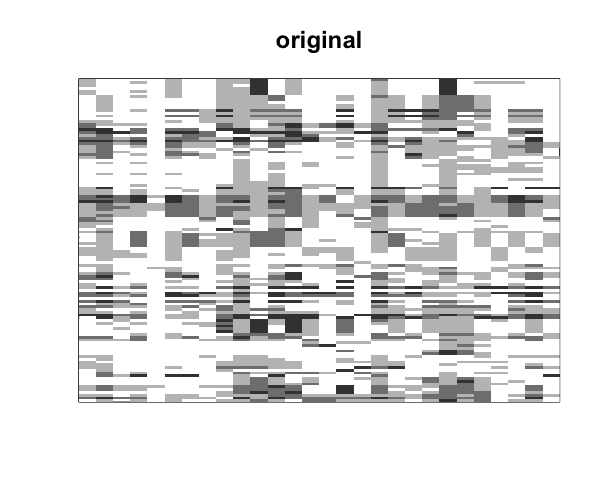
\includegraphics[width = .8\textwidth]{images/original.png}
    \caption{Plot of the dataqol dataset. The rows represent the patients, the columns represent the questions they answered to. A cell is the response of a patient to a question. The more black the cell is, the more negative the answer.}
    \label{fig:original}
\end{figure}

The purpose of clustering is to emphasize information regarding the rows of a data matrix. First, the $\boldsymbol{x}$ ordinal matrix is loaded, which corresponds to the patients' responses:
\begin{example}
set.seed(1)
x <- as.matrix(dataqol[,2:29])
\end{example}
The clustering is obtained using the \code{bosclust} function:
\begin{example}
clust <- bosclust(x = x, kr = 3, m = 4, 
            nbSEM = nbSEM, nbSEMburn = nbSEMburn, 
            nbindmini = nbindmini, init = init)
\end{example}

\noindent The outcome can be plotted using the \code{plot} function:
\begin{example}
 plot(clust)
\end{example}
\begin{figure}[ht!]
\centering
  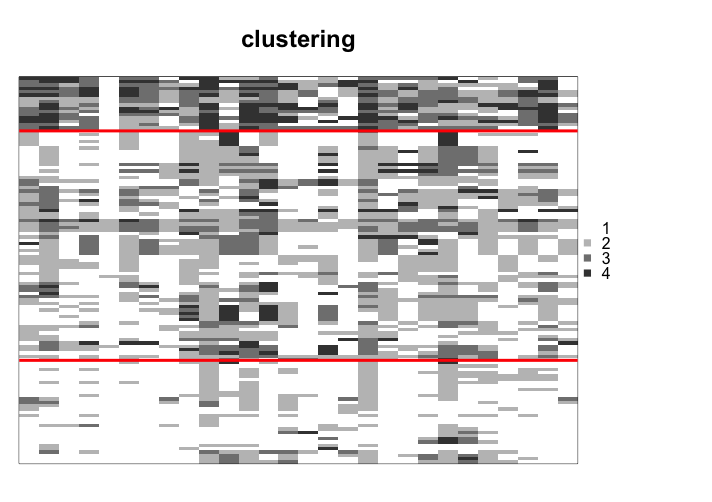
\includegraphics[width = .8\textwidth]{images/clust.png}
    \caption{Clustering obtained when following the example provided.}
    \label{fig:clust}
\end{figure}
Figure~\ref{fig:clust} represents the clustering result. We count the clusters from the bottom to the top. Among the $3$ row-clusters, the first one (at the bottom) stands out as the lightest. This means that the patients from this cluster globally chose levels close to $1$, which is the most positive answer. In contrast, the third row-cluster (at the top) is darker, which implies the patients from this group answered in a more negative way.


\paragraph{Clusters interpretation.}
The parameters are obtained with the command \code{clust@params}:
\begin{example}
> clust@params
[[1]]
[[1]]$mus
     [,1] [,2] [,3] [,4] [,5] [,6] [,7] [,8] [,9] [,10] [,11] [,12] [,13] [,14]
[1,]    1    1    1    1    1    1    1    1    1     2     1     2     1     1
[2,]    2    2    1    1    1    2    1    1    2     2     1     3     2     1
[3,]    3    4    3    3    1    4    3    2    3     4     2     4     3     4
     [,15] [,16] [,17] [,18] [,19] [,20] [,21] [,22] [,23] [,24] [,25] [,26]
[1,]     1     1     1     2     1     1     1     2     1     1     1     1
[2,]     1     1     1     2     2     1     2     2     1     2     1     1
[3,]     1     1     1     4     3     3     3     3     2     2     2     3
     [,27] [,28]
[1,]     1     1
[2,]     1     1
[3,]     4     1

[[1]]$pis
          [,1]      [,2]     [,3]      [,4] [,5]      [,6]      [,7]      [,8]
[1,] 0.8079608 0.6673682 0.961979 0.7770536    1 0.9619790 1.0000000 0.8852379
[2,] 0.3946294 0.3736864 0.722322 0.4690402    1 0.3567357 0.5546162 0.6402318
[3,] 0.4319502 0.5928978 0.347433 0.4930463    1 0.2718517 0.5888644 0.3310052
          [,9]     [,10]     [,11]     [,12]     [,13]     [,14]     [,15]
[1,] 0.9246885 0.5903583 0.6951631 0.5438752 0.9226941 0.4932884 0.8825371
[2,] 0.4767814 0.6937982 0.1481492 0.1859040 0.1176366 0.6624020 0.7916167
[3,] 0.3220447 0.7079570 0.4084469 0.5779180 0.5745136 0.1691940 0.3161048
         [,16]     [,17]     [,18]     [,19]     [,20]     [,21]     [,22]
[1,] 0.8036703 0.7364791 0.6643935 1.0000000 0.9619790 0.6951631 0.5681893
[2,] 0.3054584 0.8394348 0.5440131 0.3395749 0.4757433 0.4142450 0.3805989
[3,] 0.1255990 0.4281432 0.5470879 0.4280508 0.2300193 0.5776385 0.2632960
         [,23]     [,24]     [,25]     [,26]     [,27]     [,28]
[1,] 0.4905033 0.5510665 0.8167944 0.7477762 0.8521366 0.9226941
[2,] 0.3870155 0.4064222 0.6484691 0.4666815 0.3530825 0.6599010
[3,] 0.4183768 0.4709545 0.1959082 0.5465595 0.6419857 0.4174326
\end{example}

\noindent \code{clust@params} is a list: when the data have $D$ numbers of levels as in Figure~\ref{fig:mat-diff-m}, the list is $D-$long. Here the data has only one number of levels, so \code{clust@params} has one element. Each element of the list has two attributes, \code{pis} and \code{mus}. They indicate the $\pi$ and $\mu$ values for each row-cluster and each column. Here, we see that, as observed with Figure~\ref{fig:clust}, the first row-cluster has globally lower parameters $\mu$, which means that people from this cluster globally answered in a more positive way to the questions. We also note that the $\pi$ parameters for the fifth variable (the fifth question) are all equal to $1$. This means that the dispersion around the position $\mu$ is null. When observing the $\mu$ parameters for the fifth variables, they are also all equal to $1$. This means that everybody answered in a positive way to this question. The fifth question of the EORTC QLQ-C30 questionnaire is "Do you need help with eating, dressing, washing yourself or using the toilet?". Therefore, we know that none of the participants had problems getting ready and eating the week before they answered the questionnaire.

\paragraph{Choosing $G$.} 
In the example above, the choice for $G$ was made by performing several clustering with $G=(2,3,4)$. Using the command \code{clust@icl}, we can find out which result has the highest ICL value. The $G$ with the highest ICL-BIC was retained, that is to say $G=3$. The code to perform these clusterings is available in the Appendix~"\nameref{sec:appendix-icl-clust}".
  

\subsection{Performing co-clustering}
\label{sec:appli-coclust}

\paragraph{Co-clustering setting.} Once again, this section uses the \code{dataqol} dataset. The co-clustering is performed using the \code{boscoclust} function:
\begin{example}
set.seed(1)
coclust <- boscoclust(x = x, kr = 3, kc = 3, m = 4,
                nbSEM = nbSEM, nbSEMburn = nbSEMburn,
                nbindmini = nbindmini, init = init)
\end{example}
\noindent As in the clustering context, the result can be plotted with the command below, as in Figure~\ref{fig:coclust}.
\begin{example}
plot(coclust)
\end{example}


\begin{figure}[ht!]
\centering
  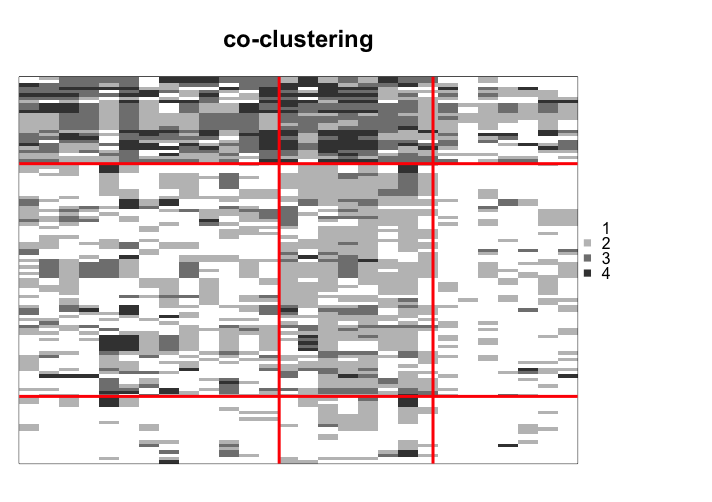
\includegraphics[width = .8\textwidth]{images/coclust.png}
    \caption{Co-clustering obtained when following the example provided.}
    \label{fig:coclust}
\end{figure}



In this case, the algorithm highlights a structure amid the rows, as for the clustering Figure~\ref{fig:clust}. In addition, it also reveals a structure inherent to the columns: for example, the third column-cluster is lighter than the others, consequently, these questions were globally responded to in a more positive way.

\paragraph{Co-clusters interpretation.} Once again, the parameters of the co-clustering are available through the command \code{coclust@params}:
\begin{example}
> coclust@params
[[1]]
[[1]]$mus
     [,1] [,2] [,3]
[1,]    1    1    1
[2,]    1    2    1
[3,]    3    3    1

[[1]]$pis
          [,1]      [,2]      [,3]
[1,] 0.8496224 0.6266097 0.9426305
[2,] 0.4876194 0.5340329 0.7722278
[3,] 0.2638594 0.3044552 0.3623779
\end{example}

In order to find out which questions belong to the third column-cluster (the one whose corresponding blocks are lighter), we need the command \code{coclust@zc}, which indicates the column-cluster of each column. \code{coclust@zc} is also a list of length $D$ (when we have different numbers of levels). Here, $D=1$ so we need \code{coclust@zc[[1]]}: 
\begin{example}
which(coclust@zc[[1]] == 3)
[1]  3  5  8 15 17 25 28
\end{example}

We know that questions 3, 5, 8, 15, 17, 25 and 28 are globally the ones that were answered the more positively. Here is the list of these questions in the EORTC QLQ C30:
\begin{itemize}
\item 3. Do you have any trouble taking a \underline{short} walk outside of the house?
\item 5. Do you need help with eating, dressing, washing yourself or using the toilet?
\item 8. During the past week, were you short of breath?
\item 15. During the past week, have you vomited??
\item 17. During the past week, have you had diarrhea?
\item 25. During the past week, have you had difficulty remembering things?
\item 28. During the past week, has your physical condition or medical treatment caused you financial difficulties?
\end{itemize}

\paragraph{Choosing $G$ and $H$.} 
In the examples above, the choice for $G$ and $H$ were made by performing several co-clusterings with $G=(2,3,4)$ and $H=(2,3,4)$. In both cases, the couple $(G,H)$ with the highest ICL-BIC value was retained, i.e., for $(G,H)=(3,3)$. The code to search the highest ICL value is given in the Appendix~"\nameref{sec:appendix-icl-coclust}"\footnote{In case of several numbers of levels, testing all the possible values for $(G,H_{1},...,H_{D})$ can be tedious. In such cases, users are invited to implement a specific heuristic strategy as in \citet{Selosse18}.}.

\subsection{Missing values.}
In this section we use the \code{dataqol} dataset. It has $1.1\%$ missing values ($40$ elements are missing in the matrix). The SEM-algorithm can handle these values since at each Expectation step (see Algorithm~\ref{algo:sem}, which computes the expectation of the missing values. The following code obtains the index of the missing values and prints their values imputed by the clustering (or co-clustering) algorithm in the Section~"\nameref{sec:appli-coclust}" (or the Section~"\nameref{sec:appli-clust}").
\begin{example}
missing <- which(is.na(x))
missing

values.imputed.clust <- clust@xhat[[1]][missing]
values.imputed.clust

values.imputed.coclust <- coclust@xhat[[1]][missing]
values.imputed.coclust
\end{example}
\begin{example}
> missing
 [1]  148  177  278  352  380  440  450  559  996 1058 1496 1513 1611 1883 1981
[16] 2046 2047 2050 2085 2285 2402 2450 2514 2517 2518 2663 2754 2785 2900 2902
[31] 2982 2986 3060 3152 3366 3367 3368 3520 3572 3602
> values.imputed.clust
 [1] 4 4 4 1 1 1 4 4 1 4 4 4 4 1 4 1 1 1 4 4 4 4 4 4 4 4 4 4 4 4 1 1 1 4 1 1 1
> values.imputed.coclust
 [1] 2 2 2 2 2 2 2 2 2 2 2 2 2 2 2 2 2 2 2 2 2 2 2 2 2 2 2 2 2 2 2 2 2 2 2 2 2
\end{example}

We see that the co-clustering and the clustering algorithm had different values imputed for the missing data.


\subsection{Comparison of clustering and co-clustering.}

\paragraph{Co-clustering as parsimonious clustering.}
Co-clustering can be seen as a parsimonious way of performing clustering, which is why these two techniques are compared here. For example, the interpretation of row-clusters is more precise with the co-clustering. Indeed, in Figure~\ref{fig:clust}, the row-clusters can be seen as a group of people who globally replied positively, a group of people who replied negatively, and a third group that replied in between. On the other hand, in Figure~\ref{fig:coclust}, an inherent structure of the data is better highlighted and adds more information: for each row-cluster, it is also easy to detect the questions that were replied to negatively. Co-clustering can therefore be seen as a more efficient way of performing clustering. Furthermore the interpretation of the parameters was easier with the co-clustering result because it only had $18$ parameters: $kr \times kc$ for $\boldsymbol\pi$ and $kr \times kc$ for $\boldsymbol\mu$. The clustering result had $168$ parameters ($kr \times J$ for $\boldsymbol\pi$ and $kr \times J$ for $\boldsymbol\mu$), which is a lot to process for the user.

\paragraph{ARI values on row partitions} The Adjusted Rand Index \citep{Rand71} was computed on row partitions of co-clustering and clustering results, using the package \CRANpkg{mclust} \cite{Fraley19}. 
\begin{example}
mclust::adjustedRandIndex(coclust@zr, clust@zr)
\end{example}
The value obtained is \code{0.41}, meaning that co-clustering creates a row partition related to that created by the clustering, without being identical.


\subsection{Setting the SEMburn and nbSEMburn arguments}
\label{sec:checkp}
The SEM-algorithm can be slow at reaching its stationary state, depending on the dataset. After having chosen arbitrary \code{nbSEM} and \code{nbSEMburn} arguments (in practice at least higher than $50$), the stability of the algorithm has to be verified. For this reason, all the functions of the \pkg{ordinalClust} package also return parameters estimations at each iteration of the SEM-algorithm. Indeed, the \code{pichain}, \code{rhochain} and \code{paramschain} slots represent the $\boldsymbol{\gamma}$, $\boldsymbol{\rho}$ and $\boldsymbol{\alpha}$ values, respectively, for each iteration. As a result, the evolution of the parameters can be analyzed and users can be confident that the returned parameters are well estimated. In the co-clustering case, for example, the evolution of the parameters can be visualized through a plot:

\begin{example}
par(mfrow=c(3,3))
for(kr in 1:3){
    for(kc in 1:3){
        toplot <- rep(0, nbSEM)
        for(i in 1:nbSEM){
            toadd <- coclust@paramschain[[1]]$pis[kr,kc,i]
            toplot <- c(toplot, toadd)
        }
        plot.default(toplot, type = "l",ylim = c(0,1), 
                 col = "hotpink3", main = "pi", 
                 ylab = paste0("pi_", kr, kc, "values"), 
                 xlab = "SEM-Gibbs iterations")
    }
}
\end{example}

\begin{figure}[ht!]
\centering
  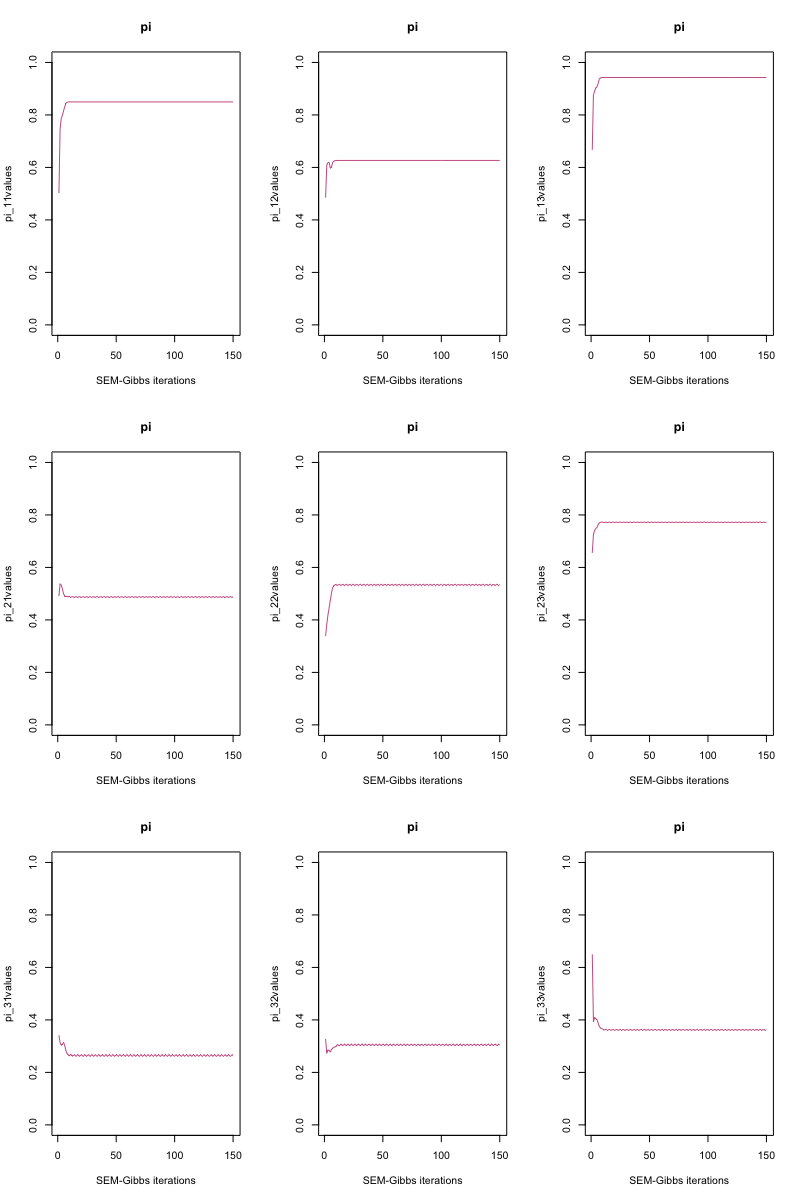
\includegraphics[width = 0.85\textwidth]{images/params-pi-evolution.png}
    \caption{Evolution of $\boldsymbol\pi$ parameters through SEM-Gibbs iterations, in the clustering example. We observe that the parameters have reached a stationary state with time.}
    \label{fig:conv}
\end{figure}
In Figure~\ref{fig:conv}, we observe that the parameters reach their stationary state before the $100^{th}$ iteration. In this case, a burn-in period of $100$ iterations (corresponding to \code{nbSEMburn=100}) is therefore enough. The total number of iterations corresponds to the argument \code{nbSEM=150}, so $50$ iterations are used to approximate the parameters.

\subsection{Handling data with different numbers of levels}
If users wish to execute one of the functions described previously on variables with different $m$, then they should use the same function with some changes to the arguments definitions. Let us assume that the data is made of $D$ different numbers of levels. First of all, the columns of matrix matrix \code{x} must be grouped by same number of levels \code{m[d]}. The additional changes for the arguments to pass are listed below:
\begin{itemize}
\item \code{m} must be a vector of length $D$. The $d^{th}$ element indicates the number of levels for the $d^{th}$ group of variables.
\item \code{kc} must be a vector of length $D$. The $d^{th}$ element indicates the number of column-clusters for the $d^{th}$ group of variables.
\item \code{idx\_list} is a new vector argument of length $D$.  The $d^{th}$ item of the vector indicates the index of the first column that have the number of levels \code{m[d]}.
\end{itemize}

An example on the \code{dataqol} dataset is available in the Appendix~"\nameref{sec:appendix-diff-m}".


\section{Conclusion}
\label{sec:conclusion}

The \pkg{ordinalClust} package presented in this paper implements several methods for analyzing ordinal data. First, it implements a clustering and co-clustering framework based on the Latent Block Model, coupled with a SEM-Gibbs algorithm and the BOS distribution. Moreover, it defines a novel approach to classify ordinal data. For the classification method, two models are proposed, so that users can introduce parsimony in their analyses. Similarly, it has been shown that the co-clustering method provides a parsimonious way of performing clustering. The framework is able to handle missing values which is notably relevant in the case of real datasets. Finally, these techniques are also implemented in the case of dataset with ordinal data with several numbers of levels.
The package \pkg{ordinalClust} is available on the Comprehensive R Archive Network (CRAN), and is still under active development. A future work will implement the method defined in \citet{gelman92}, to automatically define the number of iterations of the SEM-Gibbs algorithm. 

\newpage 


\bibliography{selosse-jacques-biernacki}


\newpage
\thispagestyle{empty}
\addcontentsline{toc}{section}{Annexe}
\section{Appendix}
\addtocontents{toc}{\protect\setcounter{tocdepth}{-1}}
\renewcommand{\thesubsection}{A\arabic{subsection}}
\setcounter{subsection}{0}

\setcounter{figure}{0}
\setcounter{table}{0}
\makeatletter 
\renewcommand{\thefigure}{A\@arabic\c@figure}
% \renewcommand{\thetable}{A\@arabic\c@table}
\makeatother

\subsection{Specificity and sensitivity}
\label{sec:appendix-spec-sens}
\noindent The following code computes the specificities, and sensitivities obtained with the different \code{kc} in the section~"\nameref{sec:classif}":

\begin{example}
library(caret)

actual <- v.validation - 1

specificities <- rep(0,length(kcol))
sensitivities <- rep(0,length(kcol))

for(i in 1:length(kcol)){
  prediction <- unlist(as.vector(preds[i,])) - 1
  u <- union(prediction, actual)
  conf_matrix <- table(factor(prediction, u),factor(actual, u))
  sensitivities[i] <- recall(conf_matrix)
  specificities[i] <- specificity(conf_matrix)
}

sensitivities
specificities
\end{example}
\begin{example}
> sensitivities
[1] 0.6666667 1.0000000 1.0000000 1.0000000 0.7777778
> specificities
[1] 0.4444444 0.5555556 0.3333333 0.5555556 0.6666667
\end{example}

\subsection{ICL search for clustering}
\label{sec:appendix-icl-clust}
\begin{example}
set.seed(1)

library(ordinalClust)
data("dataqol")
M <- as.matrix(dataqol[,2:29])

nbSEM <- 150
nbSEMburn <- 100
nbindmini <- 2
init <- "randomBurnin"
percentRandomB <- c(50)
icl <- rep(0,3)

for(kr in 2:4){
    object <- bosclust(x = M, kr = kr, m = 4, nbSEM = nbSEM,
                nbSEMburn = nbSEMburn, nbindmini = nbindmini, 
                percentRandomB = percentRandomB, init = init)

    if(length(object@icl)) icl[kr-1] <- object@icl  
}
icl
\end{example}
\begin{example}
> icl
[1] -3713.311 -3192.351 0   
\end{example}

We see that the clustering algorithm could not find a solution without an empty cluster for \code{kr = 4}. The highest icl is for \code{kr = 3}.

\subsection{ICL search for co-clustering}
\label{sec:appendix-icl-coclust}
\begin{example}
set.seed(1)
library(ordinalClust)
data("dataqol")
M <- as.matrix(dataqol[,2:29])

nbSEM <- 150
nbSEMburn <- 100
nbindmini <- 2
init <-  "randomBurnin"
percentRandomB <- c(50, 50)
icl <- matrix(0, nrow = 3, ncol = 3)

for(kr in 2:4){
    for(kc in 2:4){
        object <- boscoclust(x = M,kr = kr, kc = kc, m = 4, nbSEM = nbSEM,  
                        nbSEMburn = nbSEMburn, nbindmini = nbindmini,
                        percentRandomB = percentRandomB, init = init)
        if(length(object@zr)){
       icl[kr-1, kc-1] <- object@icl 
      } 
    }

}

icl
\end{example}
\begin{example}
> icl
          [,1]      [,2]      [,3] 
[1,] -3529.423     0.000 -3503.235    
[2,]     0.000 -3373.573     0.000    
[3,]     0.000 -3361.628 -3299.497    

\end{example}

We note that the co-clustering algorithm could not find a solution without an empty cluster for \code{(kr, kc) = (2,3), (3,2), (3,4), (4,2)}. The highest ICL-BIC is obtained when \code{(kr,kc) = (3, 3)}.

\subsection{Handling different numbers of levels}
\label{sec:appendix-diff-m}
The following code shows how to handle different numbers of levels in a co-clustering context. It may take several minutes due to the high number of levels of the two last columns.

\begin{example}
set.seed(1)

library(ordinalClust)

# loading the real dataset
data("dataqol")

# loading the ordinal data
x <- as.matrix(dataqol[,2:31])


# defining different number of categories:
m <- c(4,7)


# defining number of row and column clusters
krow <- 3
kcol <- c(3,1)

# configuration for the inference
nbSEM <- 20
nbSEMburn <- 15
nbindmini <- 2
init <- 'random'

d.list <- c(1,29)

# Co-clustering execution
object <- boscoclust(x = x,kr = krow, kc = kcol, m = m,
                idx_list = d.list, nbSEM = nbSEM,
                nbSEMburn = nbSEMburn, nbindmini = nbindmini,
                init = init)
\end{example}

\newpage 



\address{Margot Selosse\\
  Universit{\'e} de Lyon, Lyon 2, ERIC EA 3083.\\
   5 Avenue Pierre Mend{\'e}s France, 69500 Bron\\
  France\\
  %(ORCiD if desired)\\
  \email{margot.selosse@gmail.com}}

\address{Julien Jacques\\
  Universit{\'e} de Lyon, Lyon 2, ERIC EA 3083.\\
   5 Avenue Pierre Mend{\'e}s France, 69500 Bron\\
  France\\
  %(ORCiD if desired)\\
  \email{julien.jacques@univ-lyon2.fr}}

\address{Christophe Biernacki\\
  Inria, Universit{\'e} de Lille, CNRS
  Universit{\'e} Lille - UFR de Math{\'e}matiques - Cit{\'e} Scientifique - 59655 Villeneuve d'Ascq Cedex \\
  France\\
  %(ORCiD if desired)\\
  \email{christophe.biernacki@inria.fr}}
